\chapter{Open Strings, D-Branes and T-Duality}\label{ch:dbranes}

So far T-duality has been a statement about closed strings: a closed string can wind around a
circle, winding is exchanged with momentum, and the theories at radius $R$ and $\ap/R$ are the
same (\cref{ch:circle,ch:tduality}). An open string has two free ends and cannot wind: it can
always be unwound and shrunk to a point. What, then, does T-duality do to a theory that contains
open strings? This chapter answers the question, and the answer changed the subject. The dual
of an open string with freely moving ends is an open string whose ends are \emph{stuck} on a
hypersurface. The hypersurface is not part of the background that we put in by hand; it
fluctuates, it has a tension, and it carries a gauge field. It is a \emph{D-brane}. A student
should care for two reasons. First, the argument is a clean example of how a duality forces new
objects into a theory. Second, D-branes and their non-dynamical cousins, the orientifold planes,
are the sources whose charges must add up to zero on a compact space. That bookkeeping is the
\emph{tadpole condition}\index{tadpole condition} that governs the compactifications on $\KT$ studied in
\cref{ch:k3t2,ch:tadpole}.

Everything physical in this chapter is Tier~\TL: it is taken from the lectures of Polchinski
(key Pol) and Tong, and none of it is formalized in this book's Lean library.
\Cref{sec:dbranes:lean} says precisely what is and is not checked, and
\cref{sec:dbranes:formal} turns the central mechanism into two small Lean statements that a
student can prove.

\section{Open strings and their boundary conditions}\label{sec:dbranes:bc}

\subsection{The boundary term}

Take the Polyakov action in conformal gauge (\cref{ch:classical}) for a worldsheet that is a
strip, $-\infty<\tau<\infty$ and $0\le\sigma\le\pi$:
\begin{equation}\label{eq:dbranes:action}
 S=-\frac1{4\pi\ap}\int\dd\tau\int_0^\pi\dd\sigma\;\partial_\alpha X^\mu\,\partial^\alpha X_\mu ,
\end{equation}
with the index $\alpha\in\{\tau,\sigma\}$ raised by the worldsheet Minkowski metric
$\diag(-1,+1)$. Vary $X^\mu\to X^\mu+\delta X^\mu$ and integrate by parts:
\begin{equation}\label{eq:dbranes:variation}
 \delta S=\frac1{2\pi\ap}\int\dd^2\sigma\;(\partial^\alpha\partial_\alpha X_\mu)\,\delta X^\mu
 \;-\;\frac1{2\pi\ap}\int\dd\tau\,\Big[\partial_\sigma X_\mu\,\delta X^\mu\Big]_{\sigma=0}^{\sigma=\pi}
 \;+\;(\text{terms at }\tau=\pm\infty)
\end{equation}
\source{Tong §3, ll.~3040--3073; Pol §1.1, ll.~65--90}. The terms at initial and final time
vanish because $\delta X^\mu$ is held fixed there, as always in the principle of least action. The
first term gives the wave equation $\partial_+\partial_-X^\mu=0$, as for the closed string. The
second term is new. For a closed string there is no boundary and it is absent; for the open
string it must vanish separately at each end, because variations near $\sigma=0$ and near
$\sigma=\pi$ are independent:
\begin{equation}\label{eq:dbranes:bcgeneral}
 \partial_\sigma X_\mu\,\delta X^\mu=0\qquad\text{at }\sigma=0\text{ and at }\sigma=\pi .
\end{equation}
For each direction $\mu$ and each end there are two ways to satisfy
\eqref{eq:dbranes:bcgeneral} \source{Tong §3, ll.~3074--3104}.

\begin{definition}[Neumann and Dirichlet conditions]\label{def:dbranes:ND}
\index{Neumann boundary condition}\index{Dirichlet boundary condition}
The \emph{Neumann} (N) condition in the direction $\mu$ is $\partial_\sigma X^\mu=0$ at the end
of the string; $\delta X^\mu$ is unrestricted. The \emph{Dirichlet} (D) condition is
$\delta X^\mu=0$, that is, $X^\mu=c^\mu$ is a constant at the end of the string; then
$\partial_\tau X^\mu=0$ there.
\end{definition}

The two conditions say opposite things about the flow of momentum. The momentum current along
the string is $P^\sigma_\mu=-\frac1{2\pi\ap}\partial_\sigma X_\mu$ (\cref{ch:classical}), so the
Neumann condition states that no momentum flows off the end of the string. With Neumann
conditions in all directions the end is free, and one can show that it moves at the speed of
light \source{Tong §3, ll.~3078--3094}. The Dirichlet condition instead fixes the position and
lets momentum flow out: something must absorb it. The Neumann condition is the only one
compatible with Poincar\'e invariance in all $D$ dimensions \source{Pol §1.1, ll.~87--90}, because
a constant vector $c^\mu$ singles out a place.

\begin{definition}[D$p$-brane]\label{def:dbranes:Dp}\index{D-brane}
Impose Neumann conditions in the directions $a=0,1,\dots,p$ and Dirichlet conditions
$X^I=c^I$ in the directions $I=p+1,\dots,D-1$, at both ends. The ends then lie on the
$(p+1)$-dimensional hypersurface $\{X^I=c^I\}$ of spacetime, called a \emph{D$p$-brane}; $p$ is
the number of its spatial dimensions.
\end{definition}

The brane breaks the Lorentz group as $SO(1,D-1)\to SO(1,p)\times SO(D-p-1)$
\source{Tong §3, ll.~3118--3139}. A D$0$-brane is a particle, a D$1$-brane a string-like object, a
D$2$-brane a membrane. Neumann conditions in all directions are the case $p=D-1$: a
space-filling brane, so that ``the end can be anywhere'' \source{Tong §3, ll.~3150--3153}.
Dirichlet conditions in all directions, time included, describe the D-instanton\index{D-instanton} \source{Tong §3, ll.~3154--3159; Pol §1.1, ll.~109--111}.
\Cref{fig:dbranes:ND} shows the two kinds of end.

\begin{figure}[ht]
\centering
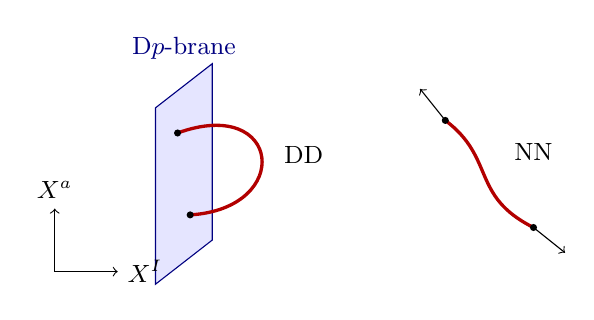
\begin{tikzpicture}[scale=0.8]
 % brane
 \fill[blue!10] (0,-1.4)--(0.9,-0.7)--(0.9,2.1)--(0,1.4)--cycle;
 \draw[blue!50!black] (0,-1.4)--(0.9,-0.7)--(0.9,2.1)--(0,1.4)--cycle;
 \node[blue!50!black] at (0.45,2.35) {\small D$p$-brane};
 % string with both ends on brane
 \draw[very thick,red!70!black] (0.35,1.0) .. controls (2.0,1.6) and (2.2,-0.2) .. (0.55,-0.3);
 \fill (0.35,1.0) circle (1.6pt); \fill (0.55,-0.3) circle (1.6pt);
 \node at (2.35,0.65) {\small DD};
 % axes
 \draw[->] (-1.6,-1.2)--(-0.6,-1.2) node[right] {\small $X^I$};
 \draw[->] (-1.6,-1.2)--(-1.6,-0.2) node[above] {\small $X^a$};
 % free string
 \draw[very thick,red!70!black] (4.6,1.2) .. controls (5.4,0.6) and (5.0,0.0) .. (6.0,-0.5);
 \draw[->,thin] (4.6,1.2)--(4.2,1.7); \draw[->,thin] (6.0,-0.5)--(6.5,-0.9);
 \fill (4.6,1.2) circle (1.6pt); \fill (6.0,-0.5) circle (1.6pt);
 \node at (6.0,0.7) {\small NN};
\end{tikzpicture}
\caption{Left: in the transverse directions $X^I$ the ends obey Dirichlet conditions and sit on
the brane; along the brane they obey Neumann conditions and slide freely. Right: with Neumann
conditions in every direction both ends are free.}\label{fig:dbranes:ND}
\end{figure}

\subsection{Mode expansions}

We solve the wave equation as $X^\mu=X^\mu_L(\sigma^+)+X^\mu_R(\sigma^-)$ with
$\sigma^\pm=\tau\pm\sigma$. We keep the conventions of \cref{ch:circle}, where the oscillators
$\tilde\alpha_k$ sit in $X_L$ and $\alpha_k$ in $X_R$, and we write $k$ for the mode number:
\begin{align}
 X_L^\mu(\sigma^+)&=\tfrac12x^\mu+\ap p^\mu\sigma^+
   +\ii\sqrt{\frac\ap2}\sum_{k\ne0}\frac1k\,\tilde\alpha^\mu_k\,\ee^{-\ii k\sigma^+},\notag\\
 X_R^\mu(\sigma^-)&=\tfrac12x^\mu+\ap p^\mu\sigma^-
   +\ii\sqrt{\frac\ap2}\sum_{k\ne0}\frac1k\,\alpha^\mu_k\,\ee^{-\ii k\sigma^-}
 \label{eq:dbranes:LR}
\end{align}
\source{Tong §3, eq.~(3.4), ll.~3160--3180}. The coefficient of $p^\mu$ is $\ap$ and not
$\frac12\ap$ as for the closed string; we shall see in a moment that this makes $p^\mu$ the
spacetime momentum when $\sigma$ runs over $[0,\pi]$ only.

\begin{proposition}[Boundary conditions on the modes]\label{prop:dbranes:modes}
For the expansion \eqref{eq:dbranes:LR} on the strip $0\le\sigma\le\pi$:
\begin{enumerate}[label=(\roman*),leftmargin=*]
\item Neumann conditions at both ends hold if and only if $\alpha_k=\tilde\alpha_k$ for all
 $k\ne0$. Then
 \begin{equation}\label{eq:dbranes:NN}
  X(\tau,\sigma)=x+2\ap p\,\tau+\ii\sqrt{2\ap}\sum_{k\ne0}\frac{\alpha_k}{k}\,
    \ee^{-\ii k\tau}\cos k\sigma .
 \end{equation}
\item Dirichlet conditions $X(\tau,0)=c$, $X(\tau,\pi)=d$ hold if and only if
 $\alpha_k=-\tilde\alpha_k$ for all $k\ne0$, the term linear in $\tau$ is absent, and the zero modes are
 replaced by a term linear in $\sigma$:
 \begin{equation}\label{eq:dbranes:DD}
  X(\tau,\sigma)=c+\frac{(d-c)}{\pi}\,\sigma-\sqrt{2\ap}\sum_{k\ne0}\frac{\alpha_k}{k}\,
    \ee^{-\ii k\tau}\sin k\sigma .
 \end{equation}
\end{enumerate}
\end{proposition}
\begin{proof}
(i) Since $\partial_\sigma=\partial_+-\partial_-$, one has
$\partial_\sigma X=\sqrt{\ap/2}\sum_k(\tilde\alpha_k\ee^{-\ii k\sigma^+}-\alpha_k\ee^{-\ii k\sigma^-})$;
the zero-mode terms cancel. At $\sigma=0$ this is
$\sqrt{\ap/2}\sum_k(\tilde\alpha_k-\alpha_k)\ee^{-\ii k\tau}$, which vanishes for all $\tau$ if and
only if $\tilde\alpha_k=\alpha_k$. With this, $\partial_\sigma X\propto\sum_k\alpha_k\ee^{-\ii k\tau}\sin k\sigma$,
which vanishes at $\sigma=\pi$ precisely because $k$ is an integer. Adding $X_L$ and $X_R$ and
using $\ee^{-\ii k\sigma^+}+\ee^{-\ii k\sigma^-}=2\ee^{-\ii k\tau}\cos k\sigma$ gives
\eqref{eq:dbranes:NN}.
(ii) Now require $\partial_\tau X=0$ at the ends. Since $\partial_\tau=\partial_++\partial_-$, the
same computation with a relative sign gives $\tilde\alpha_k=-\alpha_k$ and no term $2\ap p\tau$.
The general solution of the wave equation may still contain a term linear in $\sigma$, obtained
by giving $X_L$ and $X_R$ opposite linear terms $\pm\frac{d-c}{2\pi}\sigma^\pm$; it is fixed by the
positions of the two ends. Finally
$-\ee^{-\ii k\sigma^+}+\ee^{-\ii k\sigma^-}=2\ii\,\ee^{-\ii k\tau}\sin k\sigma$, and
$\ii\cdot\ii\sqrt{\ap/2}\cdot2=-\sqrt{2\ap}$, which gives \eqref{eq:dbranes:DD}.
\end{proof}
The mode conditions are those of \source{Tong §3, eq.~(3.5) and below, ll.~3181--3202}; the two
expansions were checked symbolically with sympy against \eqref{eq:dbranes:LR}. In both cases only
one set of oscillators survives: the boundary reflects left-movers into right-movers. An open
string has, roughly, half the degrees of freedom of a closed string. For mixed conditions, N at
one end and D at the other, see \cref{ex:dbranes:ND}.

\paragraph{Momentum.} For the Neumann expansion the total momentum is the integral of the
momentum density $P^\tau=\frac1{2\pi\ap}\partial_\tau X$:
\[
 P=\frac1{2\pi\ap}\int_0^\pi\dd\sigma\,\partial_\tau X=\frac1{2\pi\ap}\,(2\ap p)\,\pi=p ,
\]
the oscillators dropping out because $\int_0^\pi\cos k\sigma\,\dd\sigma=0$ for integer $k\ne0$
\source{Tong §3, ll.~3206--3230}. This confirms the normalization of \eqref{eq:dbranes:LR}. In a
Dirichlet direction \eqref{eq:dbranes:DD} has no momentum zero mode at all: $x^I$ is replaced by
the number $c^I$ and $p^I$ by zero. States of the open string therefore have wavefunctions that
depend only on the coordinates \emph{along} the brane \source{Tong §3.1, ll.~3231--3238}. The
fields that the open string gives rise to live on the brane.

\begin{pitfallbox}
``Momentum is not conserved in the Dirichlet directions, so the theory is inconsistent.''
Translation invariance transverse to the brane is broken by the brane, exactly as it is broken
by any heavy object placed at a point. The momentum that flows off the end of the string is
absorbed by the brane. This is possible only if the brane can recoil, that is, only if it is a
dynamical object; \cref{sec:dbranes:dynamics} shows that it is.
\end{pitfallbox}

\section{The open-string spectrum}\label{sec:dbranes:spectrum}

Quantization proceeds as for the closed string (\cref{ch:quantum}), but with one set of
oscillators $[\alpha^\mu_k,\alpha^\nu_l]=k\,\delta_{k+l,0}\,\eta^{\mu\nu}$. In light-cone gauge, with the
light-cone directions chosen along the brane, the mass of a state measured by an observer on the
brane is
\begin{equation}\label{eq:dbranes:mass}
 M^2=\frac1{\ap}\,(N-1),\qquad N=\sum_{i}\sum_{k>0}\alpha^i_{-k}\alpha^i_k ,
\end{equation}
where $i$ runs over the $D-2=24$ transverse directions, both those along the brane and those
perpendicular to it. Lorentz invariance of the quantum theory again requires $D=26$ and the
normal-ordering constant $a=1$, the same values as for the closed string \source{Tong §3.1,
ll.~3248--3290}. Compared with the closed-string formula $M^2=\frac2{\ap}(N+\tilde N-2)$ of
\cref{ch:quantum}, there is one oscillator sum instead of two and an overall factor $\frac14$ at
equal level; the factor comes from $\ap p$ versus $\frac12\ap p$ in the mode expansions. The
lowest states are as follows \source{Tong §3.1.1--3.1.2, ll.~3306--3368}.
\begin{itemize}[leftmargin=*]
\item $N=0$: a tachyon with $M^2=-1/\ap$, confined to the brane. It signals that the bosonic
 D-brane is unstable and decays into closed strings. In the type~II superstring the tachyon is
 absent for D$p$-branes with $p$ even (IIA) or odd (IIB), which are stable because they carry
 Ramond--Ramond charge \source{Tong §3.1.4, ll.~3397--3406}.
\item $N=1$, oscillator along the brane, $\alpha^a_{-1}\ket{0;p}$: a massless vector of
 $SO(1,p)$, a photon $A_a$ on the brane.\index{gauge field on a brane}
\item $N=1$, oscillator transverse to the brane, $\alpha^I_{-1}\ket{0;p}$: $D-p-1$ massless
 scalars $\phi^I$ on the brane, which form a vector of the transverse rotation group
 $SO(D-p-1)$.
\end{itemize}

\paragraph{Stretched strings.}\index{stretched string}
Take two parallel D$p$-branes at transverse positions $c^I$ and $d^I$ and a string that goes
from the first to the second. Its expansion is \eqref{eq:dbranes:DD}. The term linear in
$\sigma$ contributes to the Virasoro constraint like a momentum: $\partial_\sigma X^I=(d^I-c^I)/\pi$
plays the role that $2\ap p$ plays in \eqref{eq:dbranes:NN}. The mass formula becomes
\begin{equation}\label{eq:dbranes:stretched}
 M^2=\frac{|d-c|^2}{(2\pi\ap)^2}+\frac1{\ap}(N-1)
\end{equation}
\source{Tong §3.3, ll.~3489--3520}. The first term has a classical meaning, which is also an
independent check: a static string of length $L=|d-c|$ and tension $T=1/(2\pi\ap)$ has energy
$TL$, and $(TL)^2$ is the first term. The ground state of the stretched string is tachyonic only
if $L<2\pi\sqrt{\ap}$, that is, when the branes approach each other to within a distance of the
order of the string length.

\section{T-duality of open strings}\label{sec:dbranes:tduality}

\subsection{A paradox at small radius}

Compactify $X^{25}\sim X^{25}+2\pi R$ and consider open strings with Neumann conditions in all
directions. The momentum along the circle is quantized, $p^{25}=n/R$, and an observer in the
$25$ non-compact dimensions sees, from \eqref{eq:dbranes:mass},
\begin{equation}\label{eq:dbranes:massR}
 M^2=\frac{n^2}{R^2}+\frac1{\ap}(N-1).
\end{equation}
There is no winding term: an open string has no winding number. As $R\to0$ all states with
$n\ne0$ become infinitely heavy and no new light states appear. The open strings behave like
fields: the compact dimension disappears and they live in $D-1$ dimensions. But a theory of open
strings also contains closed strings (two ends can join), and we saw in \cref{ch:tduality} that
for closed strings the compact dimension \emph{reappears} as $R\to0$, because winding states
become light. So the closed strings live in $D$ dimensions and the open strings in $D-1$
\source{Pol §2.2, ll.~679--693}.

\begin{physicsbox}
The interior of an open string is made of the same material as a closed string, so it must still
vibrate in all $D$ dimensions of the dual spacetime. What distinguishes an open string is its
ends. The only consistent reading of the paradox is that the \emph{ends} are confined to a
$(D-1)$-dimensional hyperplane of the dual spacetime while the rest of the string is not
\source{Pol §2.2, ll.~694--697}.
\end{physicsbox}

\subsection{Neumann becomes Dirichlet}

The dual coordinate of \cref{ch:tduality} is $Y=X_L-X_R$ for the compact direction, and it obeys
\begin{equation}\label{eq:dbranes:eps}
 \partial_\tau X=\partial_\sigma Y,\qquad \partial_\sigma X=\partial_\tau Y .
\end{equation}
These relations are local on the worldsheet and hold equally on the strip. Read at the
boundary, the second one says
\begin{equation}\label{eq:dbranes:NtoD}
 \partial_\sigma X=0\ \ (\text{Neumann for }X)\quad\Longleftrightarrow\quad
 \partial_\tau Y=0\ \ (\text{Dirichlet for }Y),
\end{equation}
and the first one says the converse with $X$ and $Y$ exchanged. \emph{T-duality exchanges Neumann
and Dirichlet conditions} \source{Tong §8.3.2, ll.~11804--11825; Pol §2.2, ll.~697--700}.
\index{T-duality!of open strings} In the language of \cref{prop:dbranes:modes} the statement is
one line. The oscillators of $Y$ are $\tilde\alpha^Y_k=\tilde\alpha_k$ and $\alpha^Y_k=-\alpha_k$. Hence
\[
 \alpha_k=\tilde\alpha_k\ \ (\text{N for }X)\quad\Longleftrightarrow\quad
 \alpha^Y_k=-\tilde\alpha^Y_k\ \ (\text{D for }Y).
\]
We can also see it in the expansions. Subtracting instead of adding the two lines of
\eqref{eq:dbranes:LR} with $\alpha_k=\tilde\alpha_k$ gives
\begin{equation}\label{eq:dbranes:Y}
 Y(\tau,\sigma)=y_0+2\ap p\,\sigma+\sqrt{2\ap}\sum_{k\ne0}\frac{\alpha_k}{k}\,
   \ee^{-\ii k\tau}\sin k\sigma ,
\end{equation}
which is of the Dirichlet form \eqref{eq:dbranes:DD} (with $\alpha_k\to-\alpha_k$), where $y_0$ is
an undetermined constant and the separation of the ends is $d-c=2\pi\ap p$.

\subsection{Where the ends are}

Equation \eqref{eq:dbranes:NtoD} says that each end has a fixed value of $Y$. Are the two values
related? Integrate along the string and use \eqref{eq:dbranes:eps}:
\begin{equation}\label{eq:dbranes:ends}
 Y(\tau,\pi)-Y(\tau,0)=\int_0^\pi\dd\sigma\,\partial_\sigma Y
 =\int_0^\pi\dd\sigma\,\partial_\tau X=2\pi\ap\,p^{25}=\frac{2\pi\ap n}{R}=2\pi n\tilde R ,
 \qquad\tilde R=\frac{\ap}{R},
\end{equation}
\source{Pol §2.2, eq.~(31), ll.~701--720}. The dual coordinate lives on a circle of radius
$\tilde R$, so $2\pi n\tilde R$ is a whole number of turns: the two ends are at the \emph{same}
point of the dual circle, and the string wraps the circle $n$ times on the way. The momentum
number of the original description has become a winding number, as for closed strings. The
winding of an open string is meaningful here precisely because its ends are no longer free to
unwind it. The same argument applied to a path on a worldsheet that connects the ends of two
different strings shows that all ends lie on one and the same hyperplane \source{Pol §2.2,
ll.~720--727}. \Cref{fig:dbranes:wilson} below shows strings with $n=0$ and $n=1$ in the more
general setting of several branes.

The masses agree, as they must. In the dual picture the string has length $L=2\pi|n|\tilde R$ and
\eqref{eq:dbranes:stretched} gives
$M^2=(2\pi n\tilde R)^2/(2\pi\ap)^2+\frac1{\ap}(N-1)=n^2\tilde R^2/\ap^2+\dots=n^2/R^2+\dots$, which is
\eqref{eq:dbranes:massR}. The paradox is resolved. For $R\ll\sqrt{\ap}$ the natural variables are
the dual ones: spacetime has a large circle of radius $\tilde R$, closed strings move on all of
it, and open strings end on a D$24$-brane at one point of it.

\begin{proposition}[T-duality and brane dimension]\label{prop:dbranes:pshift}
T-duality along a circle tangent to a D$p$-brane gives a D$(p-1)$-brane localized at a point of
the dual circle. T-duality along a circle transverse to a D$p$-brane gives a D$(p+1)$-brane
wrapped on the dual circle. \TL\ \source{Pol §2.4, ll.~879--881; Tong §8.3.2, ll.~11820--11825}
\end{proposition}
\begin{proof}
A tangent direction carries the Neumann condition, which becomes Dirichlet by
\eqref{eq:dbranes:NtoD}; the number of Neumann directions drops by one. A transverse direction
carries the Dirichlet condition, and the first relation of \eqref{eq:dbranes:eps} turns it into
Neumann.
\end{proof}
Dualizing $k$ circles of the theory of freely moving open strings, which is a theory of
space-filling D$25$-branes, gives D$(25-k)$-branes. In the superstring, where T-duality exchanges
the type~IIA and IIB theories, the rule $p\mapsto p\pm1$ is consistent with the fact that IIA has
stable branes of even $p$ and IIB of odd $p$ \source{Tong §8.3.3, ll.~11828--11833}.

\begin{historybox}
Dirichlet conditions were first studied as a variant of string theory in its own right. Their
association with a hyperplane in spacetime came later, from compactifications of open strings;
it was then observed that the hyperplane is dynamical and can be produced by T-duality
\source{Pol §1.1, ll.~103--108}. Tong remarks that Dirichlet conditions were rarely considered
until the mid-1990s \source{Tong §3, ll.~3105--3111; §8.3.2, ll.~11826--11827}.
\end{historybox}

\section{Chan--Paton factors and Wilson lines}\label{sec:dbranes:wilson}

\subsection{Labels on the ends}

It is consistent with Poincar\'e and conformal invariance to let each end of an open string
carry a label $i\in\{1,\dots,N\}$ that has no dynamics of its own: its Hamiltonian vanishes, so an
end prepared in the state $i$ stays in it \source{Pol §1.2, ll.~227--240}. A state of the string is
then $\ket{k;ij}$, and a general state is a combination
$\sum_{i,j}\lambda_{ij}\ket{k;ij}$ with an $N\times N$ matrix $\lambda$, the
\emph{Chan--Paton factor}\index{Chan--Paton factor}. In an amplitude the right end of one string
must be in the same state as the left end of the next, so every open-string amplitude contains a
trace $\Tr(\lambda^1\lambda^2\cdots)$, invariant under $\lambda\mapsto U\lambda U^{-1}$ with
$U\in U(N)$. The $N^2$ massless vectors $\lambda_{ij}\,\alpha^\mu_{-1}\ket{k;ij}$ transform in the adjoint
representation, and the worldsheet symmetry $U(N)$ becomes a gauge symmetry in spacetime
\source{Pol §1.2, ll.~241--271}. In the brane language of Tong, the label says on which of $N$
coincident branes the end sits \source{Tong §3.3, ll.~3522--3540}.

\subsection{A Wilson line is a set of positions}

On a circle a gauge field can have a constant component that cannot be removed by a periodic
gauge transformation:
\begin{equation}\label{eq:dbranes:wilsonA}
 A_{25}=\frac1{2\pi R}\,\diag(\theta_1,\theta_2,\dots,\theta_N),\qquad
 W=\exp\Big(\ii\oint A_{25}\,\dd X^{25}\Big)=\diag(\ee^{\ii\theta_1},\dots,\ee^{\ii\theta_N}) .
\end{equation}
The field strength vanishes, but the holonomy $W$, the \emph{Wilson line}\index{Wilson line}, is
gauge invariant, and each $\theta_i$ is an angle defined modulo $2\pi$. For generic angles it
breaks $U(N)\to U(1)^N$. Locally $A_{25}$ is pure gauge, $A_{25}=-\ii\Lambda^{-1}\partial_{25}\Lambda$
with $\Lambda=\diag(\ee^{\ii\theta_iX^{25}/2\pi R})$. One may remove $A_{25}$ with $\Lambda$, but
$\Lambda$ is not periodic, and the price is that charged fields are no longer periodic: a string
in the state $\ket{ij}$, whose two ends have opposite charges under the $i$-th and $j$-th
$U(1)$, picks up the phase $\ee^{\ii(\theta_j-\theta_i)}$ under $X^{25}\to X^{25}+2\pi R$
\source{Pol §2.3, ll.~732--774}. A wavefunction $\ee^{\ii pX^{25}}$ with this periodicity has
\begin{equation}\label{eq:dbranes:fracp}
 p^{25}_{ij}=\frac{2\pi n+\theta_j-\theta_i}{2\pi R},\qquad n\in\Z .
\end{equation}
This is the familiar statement that a constant vector potential shifts the momentum of a charged
particle, $p\to p-qA$, here with charges $\mp1$ at the two ends.

Now repeat the computation \eqref{eq:dbranes:ends} with the fractional momentum:
\begin{equation}\label{eq:dbranes:sep}
 Y(\pi)-Y(0)=2\pi\ap\,p^{25}_{ij}=(2\pi n+\theta_j-\theta_i)\,\tilde R
\end{equation}
\source{Pol §2.3, eq.~(34), ll.~774--777}. The ends of an $ij$ string are no longer at the same
point. Up to a common additive constant, an end in the state $i$ sits at
\begin{equation}\label{eq:dbranes:position}
 \boxed{\;Y_i=\theta_i\tilde R=2\pi\ap\,(A_{25})_{ii}\;}
\end{equation}
\source{Pol §2.3, eq.~(35), ll.~779--783}. There are $N$ hyperplanes, one for each value of the
Chan--Paton label, at positions on the dual circle given by the eigenvalues of the Wilson line
(\cref{fig:dbranes:wilson}). The angle $\theta_i\in[0,2\pi)$ becomes the point
$Y_i\in[0,2\pi\tilde R)$: a gauge-theory modulus has become a geometric modulus.
\index{Wilson line!as brane position}

\begin{figure}[ht]
\centering
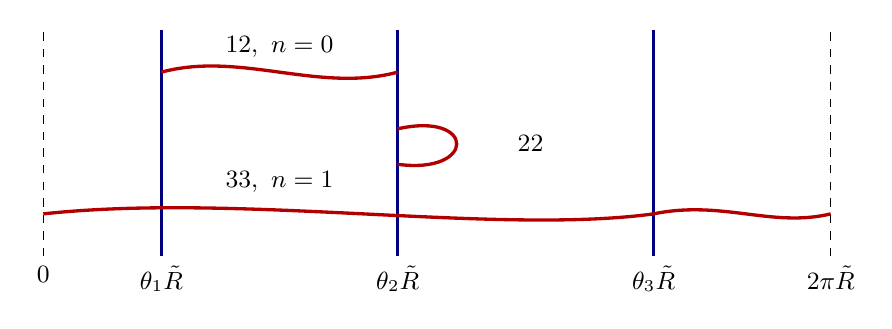
\begin{tikzpicture}[xscale=1.25,yscale=0.9]
 \draw[dashed] (0,-1.5)--(0,1.7); \draw[dashed] (8,-1.5)--(8,1.7);
 \node[below] at (0,-1.5) {\small $0$}; \node[below] at (8,-1.5) {\small $2\pi\tilde R$};
 \foreach \x/\lab in {1.2/{\theta_1\tilde R},3.6/{\theta_2\tilde R},6.2/{\theta_3\tilde R}}{
   \draw[blue!50!black,very thick] (\x,-1.5)--(\x,1.7);
   \node[below] at (\x,-1.5) {\small $\lab$};}
 % 12 string
 \draw[red!70!black,very thick] (1.2,1.1) .. controls (2.0,1.4) and (2.8,0.8) .. (3.6,1.1);
 \node at (2.4,1.45) {\small $\ket{12},\ n=0$};
 % 22 string n=0
 \draw[red!70!black,very thick] (3.6,0.3) .. controls (4.4,0.55) and (4.4,-0.35) .. (3.6,-0.2);
 \node at (4.95,0.1) {\small $\ket{22}$};
 % 33 string n=1, wraps around
 \draw[red!70!black,very thick] (6.2,-0.9) .. controls (6.9,-0.7) and (7.4,-1.1) .. (8,-0.9);
 \draw[red!70!black,very thick] (0,-0.9) .. controls (2,-0.6) and (4.6,-1.2) .. (6.2,-0.9);
 \node at (2.4,-0.45) {\small $\ket{33},\ n=1$};
\end{tikzpicture}
\caption{Three D-branes on the dual circle (the dashed lines are identified), at the positions
given by a Wilson line with angles $\theta_1,\theta_2,\theta_3$. A $\ket{12}$ string stretches
between two branes; a $\ket{22}$ string with $n=0$ can shrink to zero length; a $\ket{33}$ string
with $n=1$ winds once around the circle. After \source{Pol §2.3--2.4, Figs.~5--6,
ll.~765--800}.}\label{fig:dbranes:wilson}
\end{figure}

The spectrum confirms the picture. With \eqref{eq:dbranes:fracp} in \eqref{eq:dbranes:massR},
\begin{equation}\label{eq:dbranes:massW}
 M^2_{ij}=\Big(\frac{2\pi n+\theta_j-\theta_i}{2\pi R}\Big)^2+\frac1{\ap}(N-1)
 =\Big(\frac{(2\pi n+\theta_j-\theta_i)\,\tilde R}{2\pi\ap}\Big)^2+\frac1{\ap}(N-1)
\end{equation}
\source{Pol §2.4, eq.~(36), ll.~810--832}. The second form is \eqref{eq:dbranes:stretched} with
$L=|2\pi n+\theta_j-\theta_i|\tilde R$, the length of a string that goes from brane $i$ to brane $j$
and $n$ times around the circle. The two forms are equal because $\tilde R/\ap=1/R$. What is
Higgsing by a Wilson line in one description is the tension of a stretched string in the other.

\begin{example}[Two branes, with numbers]\label{ex:dbranes:numbers}
Work in units $\ap=1$. Let $R=\frac14$, so $\tilde R=4$ and the dual circle has circumference
$8\pi\approx25.1$. Take $N=2$ with $\theta_1=0$ and $\theta_2=\pi$: the two branes sit at
$Y_1=0$ and $Y_2=4\pi$, at diametrically opposite points. \Cref{tab:dbranes:example} lists the
lightest states at level $N=1$ (the vectors and scalars).
\begin{table}[ht]
\centering
\caption{States at oscillator level $1$ for $\ap=1$, $R=\frac14$, $\theta=(0,\pi)$. The column
$L$ is the length of the stretched string in the dual picture; the last two columns are
computed independently from the two forms of \eqref{eq:dbranes:massW}.}
\label{tab:dbranes:example}
\begin{tabular}{@{}ccccc@{}}\toprule
sector & $n$ & $L=|2\pi n+\theta_j-\theta_i|\tilde R$ & $(L/2\pi\ap)^2$ & $(p^{25}_{ij})^2$\\\midrule
$\ket{11}$, $\ket{22}$ & $0$ & $0$ & $0$ & $0$\\
$\ket{12}$ & $0$ & $4\pi$ & $4$ & $4$\\
$\ket{21}$ & $0$ & $4\pi$ & $4$ & $4$\\
$\ket{11}$, $\ket{22}$ & $\pm1$ & $8\pi$ & $16$ & $16$\\
$\ket{12}$ & $1$ & $12\pi$ & $36$ & $36$\\\bottomrule
\end{tabular}
\end{table}
There are exactly two massless vectors, $\ket{11}$ and $\ket{22}$ at $n=0$: the gauge group is
$U(1)^2$. The off-diagonal vectors, the W-bosons of the breaking $U(2)\to U(1)^2$, have mass
$M=2$, which is $(\theta_2-\theta_1)/2\pi R=\pi/(2\pi\cdot\frac14)$ in the original picture and
$TL=4\pi/2\pi$ in the dual one. The ground state of the $\ket{12}$ string has $M^2=4-1=3>0$ and is
not tachyonic, in agreement with $L=4\pi>2\pi\sqrt{\ap}$. If instead $\theta_2\to\theta_1$, the two
branes coincide, the $\ket{12}$ and $\ket{21}$ vectors become massless, and $U(2)$ is restored.
\end{example}

\section{D-branes are dynamical}\label{sec:dbranes:dynamics}

\subsection{The massless fields on the brane}

Consider the massless states of \cref{sec:dbranes:spectrum} in the T-dual picture of one
dualized circle, for a string with both ends on the brane $i$ \source{Pol §2.4,
ll.~833--854}:
\begin{equation}\label{eq:dbranes:massless}
 \alpha^\mu_{-1}\ket{k;ii},\quad V=\partial_tX^\mu;\qquad\qquad
 \alpha^{25}_{-1}\ket{k;ii},\quad V=\partial_tX^{25}=\partial_nY ,
\end{equation}
where $\partial_t$ and $\partial_n$ are the derivatives tangent and normal to the boundary of the
worldsheet, and the equality is \eqref{eq:dbranes:eps} at the boundary. The first set is a gauge
field along the brane. The second was, before dualizing, the component $A_{25}$ of the gauge
field along the circle. Equation \eqref{eq:dbranes:position} tells us what a constant value of
this field means in the dual picture: it is the \emph{position} of the brane. A value that varies
slowly along the brane, $A_{25}(\xi)$, is a brane whose transverse position
$Y(\xi)=2\pi\ap A_{25}(\xi)$ varies from place to place, that is, a brane that is bent, and
the quanta of the field are small fluctuations of its shape. This matches Tong's identification
$X^I(\xi)=2\pi\ap\,\phi^I(\xi)$ of the transverse scalars $\phi^I$ \source{Tong §3.2,
ll.~3446--3456}.

\begin{physicsbox}[The same logic as for gravity]
In \cref{ch:quantum,ch:backgrounds} we started with strings in flat spacetime, found a massless
closed-string state, and recognized it as a fluctuation of the geometry: the background is
dynamical. Here we start with a flat hyperplane, find a massless open-string state, and
recognize it as a fluctuation of the shape of the hyperplane. In a theory with gravity there
could be no perfectly rigid object anyway \source{Pol §2.4, ll.~805--809, 848--857}.
\end{physicsbox}

\paragraph{Coincident branes.}\index{coincident branes} When no two of the $N$ branes coincide, the massless vectors are
the $N$ states $\ket{ii}$ and the gauge group is $U(1)^N$. If $m$ branes coincide,
$\theta_1=\dots=\theta_m$, the strings stretched between them have zero length, there are $m^2$
massless vectors, and the gauge group is enhanced to $U(m)$; in the original description the
Wilson line leaves $U(m)$ unbroken. At the same time $m^2$ massless scalars appear: the $m$
positions are promoted to an $m\times m$ matrix \source{Pol §2.4, ll.~860--871; Tong §3.3,
ll.~3527--3549}.\index{enhanced gauge symmetry!coincident branes} In \cref{ch:tduality} the closed-string gauge symmetry was enhanced at a special radius; here
the open-string gauge symmetry is enhanced at special brane positions.

\subsection{The action and the tension}

A dynamical object needs an action. Lorentz and reparametrization invariance fix the leading
term to be the volume of the worldvolume, as for the Nambu--Goto string of \cref{ch:classical}:
the \emph{Dirac action}\index{Dirac action} $S=-T_p\int\dd^{p+1}\xi\,\sqrt{-\det\gamma_{ab}}$, with
$\gamma_{ab}=\partial_aX^\mu\partial_bX^\nu\eta_{\mu\nu}$ the induced metric and $T_p$ the tension
\source{Tong §3.2, eq.~(3.6), ll.~3417--3440}. Including the gauge field on the brane and the
closed-string background fields $G$, $B$ and the dilaton $\Phi$ of \cref{ch:backgrounds}, the
low-energy action is
\begin{equation}\label{eq:dbranes:DBI}
 S_p=-T_p\int\dd^{p+1}\xi\;\ee^{-\Phi}\sqrt{-\det\big(G_{ab}+B_{ab}+2\pi\ap F_{ab}\big)}
\end{equation}
\TL\ \source{Pol §2.5, eq.~(38), ll.~886--898}, the Dirac--Born--Infeld
action\index{Born--Infeld action}; $G_{ab}$ and $B_{ab}$ are pulled back to the brane. (Polchinski
writes $\det^{1/2}$ without the sign; the minus sign under the root is needed in Lorentzian
signature.) Three features can be understood with the tools of this chapter.
\begin{itemize}[leftmargin=*]
\item The factor $\ee^{-\Phi}=1/g_s$ appears because the action arises from the disk, the
 tree level of open strings. A D-brane is therefore heavy at weak coupling.
\item The dependence on $F$ follows from T-duality. Let the brane extend along $X^1,X^2$ with
 constant $F_{12}$, in the gauge $A_2=X^1F_{12}$. Dualize $X^2$. By
 \eqref{eq:dbranes:position} the dual brane sits at $Y^2=2\pi\ap X^1F_{12}$: it is a tilted
 brane of one dimension less. Its length element is
 $\dd X^1\sqrt{1+(\partial_1Y^2)^2}=\dd X^1\sqrt{1+(2\pi\ap F_{12})^2}$, which is
 $\sqrt{\det(\delta_{ab}+2\pi\ap F_{ab})}$ for a $2\times2$ antisymmetric $F$ \source{Pol §2.5,
 eqs.~(39)--(40), ll.~899--915}. A magnetic field on a brane is T-dual to a tilt.
\item Only the combination $B+2\pi\ap F$ can appear. The worldsheet couplings are
 $\frac1{2\pi\ap}\int_MB+\int_{\partial M}A$; the transformation $\delta B=\dd\zeta$ produces a
 boundary term which is cancelled by $\delta A=-\zeta/2\pi\ap$, and $B+2\pi\ap F$ is the
 invariant \source{Pol §2.5, eq.~(41), ll.~915--933}.
\end{itemize}

T-duality also relates the tensions of branes of different dimension. Wrap a D$p$-brane on a
torus with radii $R_1,\dots,R_p$. Its mass is $T_p\,\ee^{-\Phi}\prod_{i=1}^p2\pi R_i$. Dualize the
circle $R_p$. By \cref{prop:dbranes:pshift} the same object is a D$(p-1)$-brane wrapped on the
remaining circles, with mass $T_{p-1}\ee^{-\tilde\Phi}\prod_{i=1}^{p-1}2\pi R_i$. The couplings are
related by the dilaton shift of \cref{ch:tduality},
$\ee^{\tilde\Phi}=\ee^{\Phi}\sqrt{\ap}/R_p$. Equating the two masses,
\[
 T_p\,\ee^{-\tilde\Phi}\,\frac{\sqrt{\ap}}{R_p}\,2\pi R_p=T_{p-1}\,\ee^{-\tilde\Phi}
 \qquad\Longrightarrow\qquad
\]
\begin{equation}\label{eq:dbranes:recursion}
 \boxed{\;T_{p-1}=2\pi\sqrt{\ap}\;T_p\;}
\end{equation}
\TL\ \source{Pol §2.5, eqs.~(42)--(44), ll.~934--973; dilaton: §2.1, eq.~(30), ll.~662--668}. Dimensional analysis agrees: $T_p$ is a
mass per unit $p$-volume, so $T_{p-1}/T_p$ is a length, and the only length available is
$\sqrt{\ap}$. The radius $R_p$ has dropped out, as it must. The absolute normalization requires a one-loop computation, the
exchange of closed strings between two branes \source{Pol §2.6, ll.~990--1011}, which we do not
reproduce.

\section{Orientifolds and tadpoles: a look ahead}\label{sec:dbranes:orientifold}

The constructions of \cref{ch:k3t2,ch:tadpole} need one more object, and it arises in the same
way. An \emph{unoriented}\index{unoriented string} string theory is obtained by keeping only states invariant under
worldsheet parity $\Omega$, which exchanges left- and right-movers, $X_L\leftrightarrow X_R$.
What does $\Omega$ do to the dual coordinate? Since $Y=X_L-X_R$,
\begin{equation}\label{eq:dbranes:omega}
 \Omega:\qquad Y(\tau,\sigma)\longmapsto-Y(\tau,\pi-\sigma) .
\end{equation}
In the dual description $\Omega$ is worldsheet parity \emph{combined with} the spacetime
reflection $Y\to-Y$. Projecting onto invariant states therefore does not remove half of the
states at each point. It relates the state of a string at $Y$ to that of the orientation-reversed
string at $-Y$. The dual spacetime is the circle modulo the reflection, the interval
$0\le Y\le\pi\tilde R$, and the two fixed points $Y=0$ and $Y=\pi\tilde R$ are the locations of
\emph{orientifold planes}\index{orientifold plane}. With $k$ dualized circles the dual space is
$T^k/\Z_2$, which has $2^k$ fixed planes \source{Pol §2.7, ll.~1211--1250}. For $k=4$ this
quotient is the orbifold limit of a K3 surface (\cref{ch:kummer}), and for $k=2$ it is the base of
the $\KT$ orientifolds discussed in \cref{ch:k3t2}.

Three facts about orientifold planes matter later \source{Pol §2.7, ll.~1250--1283}.
\begin{itemize}[leftmargin=*]
\item They are not dynamical. No string states are tied to them, so they have no fluctuations
 of shape, unlike D-branes.
\item Away from the fixed planes the local physics is that of the oriented theory. Each D-brane
 at $Y_i=\theta_i\tilde R$ has an image at $-Y_i$; a Wilson line of $SO(N)$ has eigenvalue angles
 $\{\theta_1,-\theta_1,\dots,\theta_{N/2},-\theta_{N/2}\}$. There are $\frac12N$ independent branes
 for an $N$-valued Chan--Paton label.
\item When $m$ branes coincide away from a fixed plane the gauge group is $U(m)$; when they sit
 on a fixed plane, strings to the images also become massless and the group is $SO(2m)$.
\end{itemize}
Like D-branes, orientifold planes are sources for the closed-string fields: they have a tension
and, in the superstring, a Ramond--Ramond charge. For the type~II orientifold with $9-p$
dualized circles the charge of one plane is $\mp2^{p-5}$ in units of the D$p$-brane charge
$\mu_p$, and there are $2^{9-p}$ planes, so the total is
\begin{equation}\label{eq:dbranes:sixteen}
 2^{9-p}\cdot\big(\mp2^{p-5}\big)\mu_p=\mp16\,\mu_p ,
\end{equation}
independent of $p$ \TL\ \source{Pol Lecture~3, eq.~(93), ll.~1968--1984}. Now the key point. On a
compact space the lines of flux that leave a charge have nowhere to go; Gauss's law forces the
total charge to vanish. A net tension would merely make the background evolve; a net
Ramond--Ramond charge makes the field equations inconsistent. With the negative sign the charge
of the planes is cancelled by exactly $16$ D-branes (plus their $16$ images), which is the T-dual
description of the type~I string with gauge group $SO(32)$ \source{Pol Lecture~3, ll.~1985--1990}. The
corresponding count for the bosonic string is $2^{25-p}\cdot2^{p-13}=2^{12}$ branes
\source{Pol §2.7, eq.~(66) and below, ll.~1424--1443}.

\begin{physicsbox}[Why this is called a tadpole]
A source with nothing to absorb its flux shows up in perturbation theory as a diagram in which a
massless closed string is emitted into the vacuum: a one-point function, or ``tadpole''. Its
cancellation is the requirement that such one-point functions add up to zero. In
\cref{ch:tadpole} the same Gauss law appears for D$3$-brane charge, where the curvature of the
compact space itself contributes $\chi/24$ and fluxes and branes make up the balance. The logic
is the one met here: \emph{on a compact space, count all sources of a given charge, with signs,
and demand zero}.
\end{physicsbox}

\begin{pitfallbox}
Do not count branes and Chan--Paton indices as the same thing in an orientifold. There are $16$
dynamical D-branes on the interval but a $32$-valued label, because each brane has an image.
Sources, and the Lean files of this project's older libraries, normalize charges per brane, per
brane--image pair or per fixed plane; before comparing two tadpole sums, check the unit
(\cref{ch:tadpole}).
\end{pitfallbox}

\section{What the machine has checked}\label{sec:dbranes:lean}

Nothing in this chapter has been formalized. The project's Lean libraries contain no
definition of an open string, a boundary condition, a Chan--Paton factor, a Wilson line or a
D-brane as a boundary condition, and the catalogue of compiled declarations has no module on
these topics. Every physical statement above is \TL, with the source indicated. We say this
plainly because the neighbouring chapters do contain kernel-checked statements, and the
open-string story does not inherit their status. What the library does contain is the following.

\begin{leanbox}[Adjacent results in the library]
The closed-string ancestor of \eqref{eq:dbranes:NtoD} is the sign flip of the right-moving zero
mode, proved in \lean{StringTheoryFormalization/UseCases/TDualityMassSpectrum.lean} (namespace
\lean{StringTheory.UseCases.TDuality}) and discussed in \cref{ch:tduality}:
\begin{leancode}
def rightMomentum (n w R : ℚ) : ℚ := n / R - w * R

theorem tduality_flips_right_momentum (n w R : ℚ) (hR : R ≠ 0) :
    rightMomentum w n (1 / R) = - rightMomentum n w R := by ...
\end{leancode}
\textbf{Reading.} For rational numbers $n,w,R$ with $R\ne0$, exchanging the first two arguments
and replacing $R$ by $1/R$ negates the function $n/R-wR$. This is the zero-mode part of
``T-duality reflects the right-movers'' at $\ap=1$. It says nothing about oscillators, about a
worldsheet with boundary, or about open strings.

On the other side of this chapter, \lean{DualScaleStream2.Flux.tadpole\_budget} (file
\lean{DualScaleStream2/Flux/Tadpole.lean}, discussed in \cref{ch:tadpole}) states that for natural
numbers with $\mathit{flux}+n=24$ one has $n\le24$, and $n=24$ if $\mathit{flux}=0$. It is an
arithmetic shadow of a charge-cancellation condition and models neither branes nor Gauss's law.
\end{leanbox}

\begin{table}[ht]
\centering
\caption{Status of the main statements of this chapter.}\label{tab:dbranes:tiers}
\small\begin{tabular}{@{}p{0.56\textwidth}cl@{}}\toprule
Statement & Tier & Where\\\midrule
N/D conditions on modes; spectrum; stretched strings & \TL & Tong §3\\
T-duality exchanges N and D; $p\mapsto p\pm1$ & \TL & Pol §2.2, Tong §8.3.2\\
Wilson line $=$ brane positions \eqref{eq:dbranes:position} & \TL & Pol §2.3\\
Branes are dynamical; DBI action; $T_{p-1}=2\pi\sqrt{\ap}\,T_p$ & \TL & Pol §2.4--2.5\\
Orientifold planes; $16$ branes cancel the charge \eqref{eq:dbranes:sixteen} & \TL & Pol §2.7, §3\\
Closed strings, over $\Q$: \lean{tduality\_flips\_right\_momentum} & \TA & \cref{ch:tduality}\\
Statements of \cref{sec:dbranes:formal} & exercise & not in the library\\\bottomrule
\end{tabular}
\end{table}

\section{A formalization exercise}\label{sec:dbranes:formal}

What would a first honest formalization of this chapter look like? The central mechanism,
\eqref{eq:dbranes:NtoD} in the form given below it, is a statement about \emph{mode data}: two
families of amplitudes, an involution that negates one of them, and two predicates exchanged by
the involution. None of this needs analysis, Hilbert spaces or a worldsheet. It is therefore a
realistic target for a student who has read \cref{ch:leanprimer}. We propose two statements.
Both were elaborated by the author against the project's toolchain and Mathlib in a scratch file.
They are \emph{not} part of the compiled library or its catalogue: in this book's bookkeeping
they are exercises, not Tier~A results.

\paragraph{Statement 1: the boundary-condition involution.}
\begin{leancode}
/-- Oscillator amplitudes of one free boson on the strip, by mode number k. -/
structure ModeData where
  left  : ℤ → ℂ      -- left-movers  (alpha-tilde_k in the text)
  right : ℤ → ℂ      -- right-movers (alpha_k in the text)

/-- T-duality: reflect the right-movers. -/
def tdual (m : ModeData) : ModeData := ⟨m.left, fun k => - m.right k⟩

def IsNeumann (m : ModeData) : Prop := ∀ k, m.right k = m.left k

def IsDirichlet (m : ModeData) : Prop := ∀ k, m.right k = - m.left k

theorem tdual_involutive (m : ModeData) : tdual (tdual m) = m := by sorry

theorem neumann_iff_dirichlet_tdual (m : ModeData) :
    IsNeumann m ↔ IsDirichlet (tdual m) := by sorry
\end{leancode}
In words: reflecting the right-movers twice is the identity, and a configuration satisfies the
Neumann relation of \cref{prop:dbranes:modes} if and only if its reflection satisfies the
Dirichlet relation. The first proof is a case split on the structure followed by \lean{simp};
the second unfolds the definitions and uses that negation is injective. The statement is
deliberately modest. It identifies \texttt{ModeData} with nothing physical; the identification
of $\alpha_k,\tilde\alpha_k$ with the modes of a string, and the derivation of the two relations
from $\partial_\sigma X=0$ and $\partial_\tau X=0$, remain \TL.

\paragraph{Statement 2: Wilson lines and positions.} The second target is the arithmetic core of
\eqref{eq:dbranes:sep} and \eqref{eq:dbranes:massW}; the real parameter \lean{a} stands for $\ap$.
\begin{leancode}
noncomputable def wilsonMomentum (n : ℤ) (θi θj R : ℝ) : ℝ :=
  (2 * Real.pi * n + θj - θi) / (2 * Real.pi * R)

theorem endpoint_separation (n : ℤ) (θi θj R a : ℝ) (hR : R ≠ 0) :
    2 * Real.pi * a * wilsonMomentum n θi θj R
      = (2 * Real.pi * n + θj - θi) * (a / R) := by sorry

theorem stretched_mass_eq_momentum (n : ℤ) (θi θj R a : ℝ)
    (hR : R ≠ 0) (ha : a ≠ 0) :
    ((2 * Real.pi * n + θj - θi) * (a / R) / (2 * Real.pi * a)) ^ 2
      = (wilsonMomentum n θi θj R) ^ 2 := by sorry
\end{leancode}
In words: $2\pi\ap$ times the fractional momentum equals the angle difference times the dual
radius $\ap/R$; and the squared energy of a classical string of that length and tension
$1/2\pi\ap$ equals the squared momentum. Both close with \lean{unfold}, the fact
\lean{Real.pi\_ne\_zero} and \lean{field\_simp}. Note which hypotheses are needed: $R\ne0$ in
both, $\ap\ne0$ only in the second, and positivity nowhere.

\paragraph{What a faithful formalization would need.} In increasing order of difficulty: (i) a
type of boundary conditions for $D$ directions, a function \lean{Fin D → Bool}, with T-duality
along direction $i$ flipping the $i$-th entry, and the theorem that the number of Neumann
directions changes by exactly one (\cref{prop:dbranes:pshift}; see \cref{ex:dbranes:leanflip});
(ii) the solution space of the wave equation on the strip, with the theorem that the Neumann
and Dirichlet conditions on smooth solutions are \emph{equivalent} to the mode relations, which
is \cref{prop:dbranes:modes} and needs Fourier series on an interval; (iii) the Fock space of the
oscillators and the mass operator, so that \eqref{eq:dbranes:massW} becomes a statement about a
spectrum and not only about its zero-mode part; (iv) the identification of a Wilson line as a
flat connection on a circle, with holonomy in a maximal torus of $U(N)$, and the map from
holonomies to configurations of $N$ points on the dual circle modulo permutations. Step (i) is
an afternoon; (ii) and (iii) are projects; (iv) needs moduli of flat connections. The count
\eqref{eq:dbranes:sixteen} is elementary arithmetic, but a faithful formalization would have to
derive the charge of an orientifold plane from an amplitude, which is far out of reach.

\begin{summarybox}
\begin{itemize}[leftmargin=*]
\item The boundary term of the open-string action vanishes for Neumann conditions
 $\partial_\sigma X=0$ (free end, no momentum flow) or Dirichlet conditions $X=c$ (fixed end). On
 the modes: $\alpha_k=\tilde\alpha_k$, respectively $\alpha_k=-\tilde\alpha_k$ with no momentum zero mode.
\item Ends with Dirichlet conditions in $D-p-1$ directions lie on a D$p$-brane. The spectrum
 $M^2=(N-1)/\ap$ contains a photon on the brane and one massless scalar per transverse
 direction. A string stretched over a distance $L$ has the extra term $(L/2\pi\ap)^2$.
\item T-duality, $X=X_L+X_R\mapsto Y=X_L-X_R$, exchanges $\partial_\sigma$ and $\partial_\tau$ and
 therefore Neumann and Dirichlet conditions. It maps D$p$ to D$(p\mp1)$ for a circle tangent
 or transverse to the brane. Open-string momentum $n/R$ becomes winding between the ends,
 $\Delta Y=2\pi n\tilde R$.
\item A Wilson line $\diag(\theta_i)/2\pi R$ becomes brane positions $Y_i=\theta_i\tilde R$;
 symmetry breaking is the mass of stretched strings, and coincident branes give $U(m)$.
\item The scalar that is T-dual to $A_{25}$ moves the brane: D-branes are dynamical, with action
 \eqref{eq:dbranes:DBI} and tensions related by $T_{p-1}=2\pi\sqrt{\ap}\,T_p$.
\item For unoriented strings T-duality produces orientifold planes at the fixed points of
 $T^k/\Z_2$. They are not dynamical but carry charge. On a compact space the total charge must
 vanish, which fixes the number of branes ($16$ plus images in type~I). This Gauss-law counting is
 the prototype of the tadpole conditions of \cref{ch:tadpole}.
\item All of this is \TL. Nothing about open strings is kernel-checked in this book's library;
 \cref{sec:dbranes:formal} proposes first targets.
\end{itemize}
\end{summarybox}

\section*{Exercises}
\addcontentsline{toc}{section}{Exercises}

\begin{exercise}[$\star$]\label{ex:dbranes:first}
Derive \eqref{eq:dbranes:variation} from \eqref{eq:dbranes:action}, keeping track of every sign.
Why is ``Neumann at one end, Dirichlet at the other'' an allowed choice?
\end{exercise}

\begin{exercise}[$\star$]
In units $\ap=1$ take $R=\frac12$ and three branes with Wilson-line angles
$\theta=(0,\frac{2\pi}3,\frac{4\pi}3)$. Find the positions of the branes on the dual circle, and the
masses of all level-one states with $M^2\le4$, once from each form of
\eqref{eq:dbranes:massW}. What is the unbroken gauge group? Is any ground state tachyonic apart
from those of the $\ket{ii}$ strings with $n=0$?
\end{exercise}

\begin{exercise}[$\star\star$]\label{ex:dbranes:ND}
Consider a direction with a Neumann condition at $\sigma=0$ and a Dirichlet condition
$X=c$ at $\sigma=\pi$. Show that the mode relation at $\sigma=0$ is still
$\alpha_k=\tilde\alpha_k$, but that the condition at $\sigma=\pi$ now forces the mode numbers to be
half-integers, $k\in\Z+\frac12$, and that there is neither a momentum nor a stretching term.
Write the analogue of \eqref{eq:dbranes:NN}. What does T-duality along this direction do to the
pair of conditions?
\end{exercise}

\begin{exercise}[$\star\star$]
A D$1$-brane is wrapped on the diagonal of a square two-torus with radii $R_1=R_2=R$, along
$X^2=X^1$. Dualize the direction $X^2$. Using \eqref{eq:dbranes:position} backwards, show that
the result is a D$2$-brane wrapped on the dual torus carrying a constant field strength, and
find $2\pi\ap F_{12}$. Check that the flux $\frac1{2\pi}\int F$ through the dual torus is an
integer. What is this integer for a brane along $X^2=qX^1$ with $q\in\Z$?
\end{exercise}

\begin{exercise}[$\star\star$]
Iterate \eqref{eq:dbranes:recursion} to express $T_p$ in terms of $T_0$. A D$p$-brane is wrapped on
a $p$-torus with all radii equal to $R$. Show that at fixed $T_0$ and fixed coupling its mass is
$T_0\ee^{-\Phi}(R/\sqrt{\ap})^p$, and interpret the result at the self-dual radius. Then verify
that the mass is unchanged if \emph{all} $p$ circles are dualized, provided the dilaton is shifted
$p$ times.
\end{exercise}

\begin{exercise}[$\star\star$, Lean]
Prove \lean{tdual\_involutive} and \lean{neumann\_iff\_dirichlet\_tdual} of
\cref{sec:dbranes:formal}. Then define the level of a finitely supported configuration as a
finite sum of products \lean{m.right (-k) * m.right k} and show that it is invariant under
\lean{tdual}. Which property of the integrand do you use, and where did it appear in
\cref{ch:tduality}?
\end{exercise}

\begin{exercise}[$\star\star$, Lean]\label{ex:dbranes:leanflip}
Let \lean{bc : Fin D → Bool} record the boundary conditions, with \lean{true} for Neumann. Define
\lean{flip i bc := Function.update bc i (!bc i)} and
\texttt{numNeumann bc := (Finset.univ.filter fun j => bc j = true).card}. State and prove: if
\lean{bc i = true} then \lean{numNeumann (flip i bc) + 1 = numNeumann bc}, and the analogous
statement for \lean{bc i = false}. Show also that \lean{flip i} is an involution. This is
\cref{prop:dbranes:pshift} as combinatorics.
\end{exercise}

\begin{exercise}[$\star\star\star$]
In the unoriented theory on the interval $0\le Y\le\pi\tilde R$, place $m$ branes at a generic
point $Y_0$ (with their images at $-Y_0$) and move them to the fixed plane $Y=0$. Using
\eqref{eq:dbranes:stretched}, list the strings that become massless in the limit and count the
massless vectors, given that the projection $\Omega$ keeps the antisymmetric combinations of
brane--image strings in the $SO$ case. Show that the count goes from $m^2=\dim U(m)$ to
$m(2m-1)=\dim SO(2m)$. Then explain why $m+\frac12$ branes can sit at a fixed plane
\source{Pol §2.7, ll.~1262--1283}.
\end{exercise}

\section*{Further reading}
\addcontentsline{toc}{section}{Further reading}
\begin{itemize}[leftmargin=*]
\item Open strings, boundary conditions, the spectrum on a brane, the Dirac action and multiple
 branes: \source{Tong §3, ll.~3040--3549}. T-duality for open strings in one page:
 \source{Tong §8.3.2--8.3.3, ll.~11804--11833}.
\item The route followed in this chapter, from Neumann conditions through T-duality to D-branes,
 Chan--Paton factors, Wilson lines, brane dynamics and the Born--Infeld action:
 \source{Pol §1.1--1.2, ll.~60--271; §2.1--2.5, ll.~482--989}.
\item Orientifolds and the cancellation of the total charge: \source{Pol §2.7, ll.~1211--1300,
 1424--1443; Lecture~3, ll.~1968--2007}.
\item In this book: the closed-string dual coordinate in \cref{ch:tduality}; the worldsheet
 derivation of T-duality in \cref{ch:buscher}; the orbifold $T^4/\Z_2$ in \cref{ch:kummer}; branes,
 fluxes and tadpoles on $\KT$ in \cref{ch:k3t2,ch:tadpole}; how to write the Lean exercises in
 \cref{ch:leanprimer}.
\end{itemize}
